

\documentclass[tikz,border=8pt]{standalone}
\usepackage{xcolor}
\usetikzlibrary{arrows.meta,positioning,shapes.geometric,calc}

\tikzset{
  actor/.style={draw=black,rounded corners=3pt,fill=gray!10,align=center,minimum width=24mm,minimum height=10mm},
  process/.style={draw=black,rounded corners=3pt,fill=blue!8,align=center,minimum width=34mm,minimum height=11mm},
  data/.style={draw=black,ellipse,fill=green!10,align=center,minimum width=34mm,minimum height=12mm},
  log/.style={draw=black,dashed,rounded corners=3pt,fill=orange!12,align=center,minimum width=34mm,minimum height=10mm},
  note/.style={draw=black,rounded corners=2pt,fill=yellow!18,align=left,minimum width=68mm,text width=68mm},
  arrow/.style={-{Latex[length=3mm]},thick,draw=black}
}

\begin{document}
\vspace*{0mm}
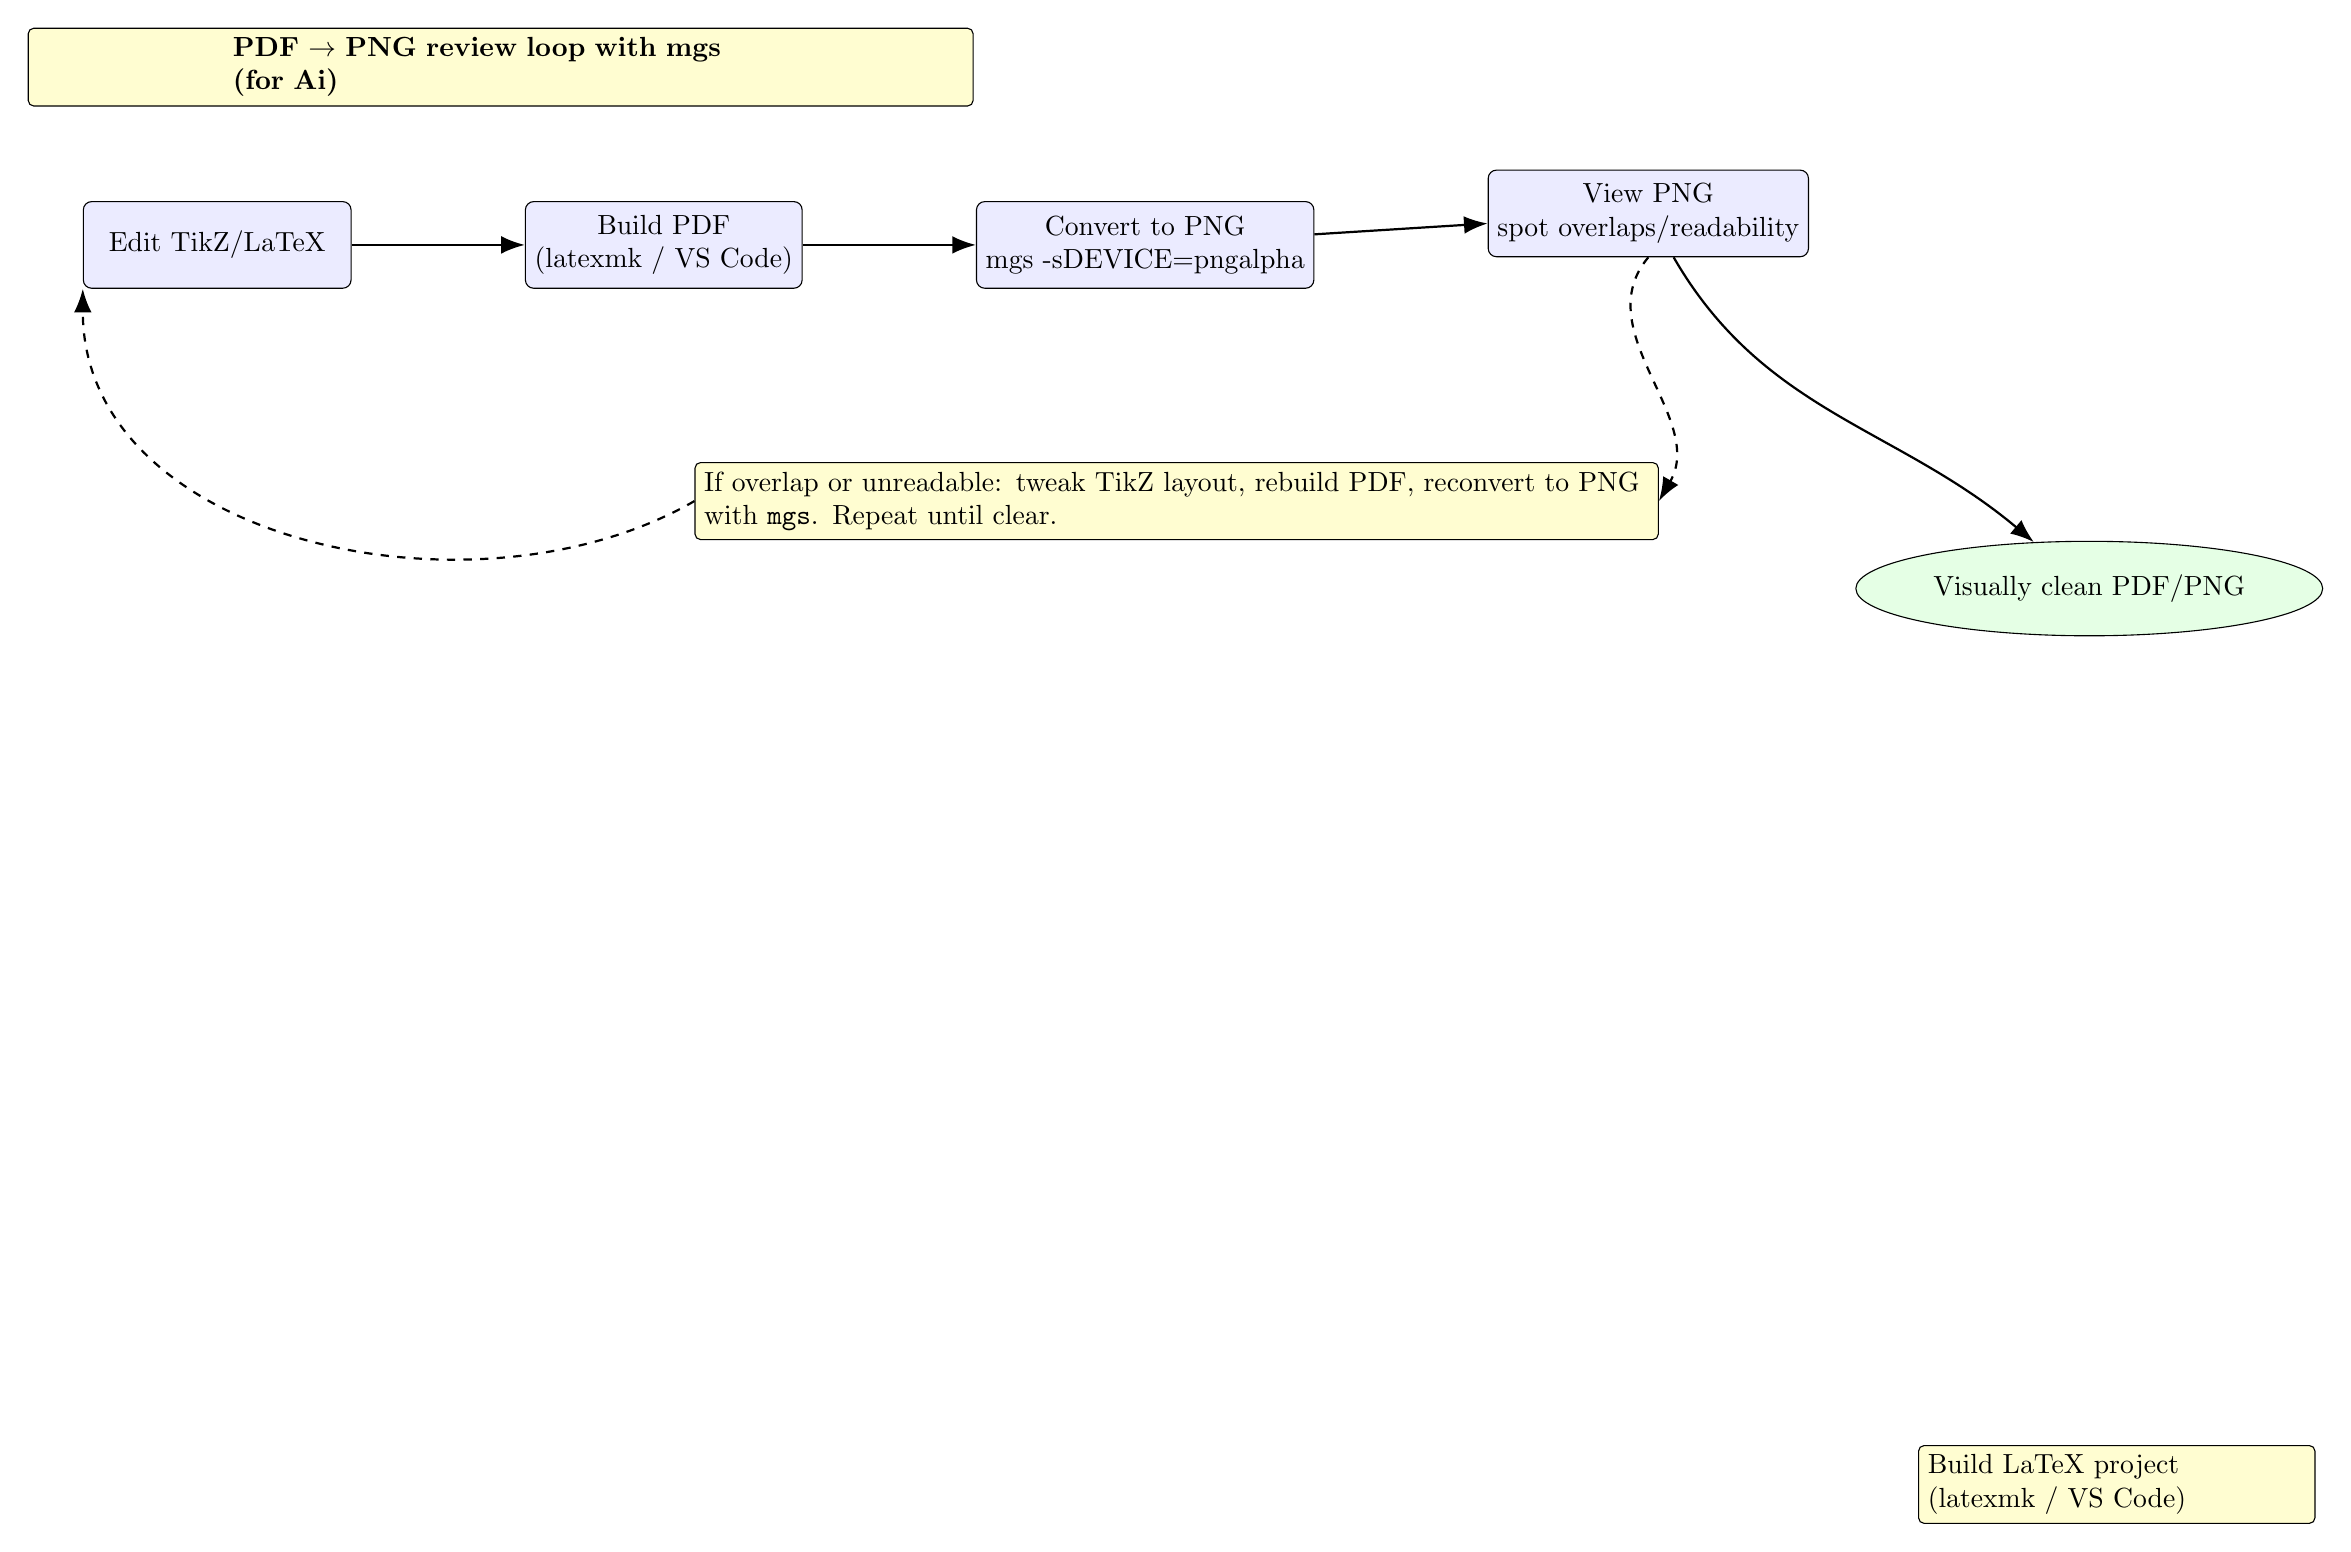
\begin{tikzpicture}[node distance=12mm,yshift=-5mm]
  \node (title3) [note,minimum width=120mm] {\textbf{PDF \(\rightarrow\) PNG review loop with mgs (for Ai)}};

  \node (edit) [process,below=of title3,xshift=-36mm] {Edit TikZ/LaTeX};
  \node (buildpdf) [process,right=22mm of edit] {Build PDF \\ (latexmk / VS Code)};
  \node (mgsnode) [process,right=22mm of buildpdf] {Convert to PNG \\ mgs -sDEVICE=pngalpha};
  \node (view) [process,right=22mm of mgsnode,yshift=4mm] {View PNG \\ spot overlaps/readability};
  \node (fixloop) [note,below=22mm of mgsnode,xshift=4mm,minimum width=120mm,text width=120mm] {If overlap or unreadable: tweak TikZ layout, rebuild PDF, reconvert to PNG with \texttt{mgs}. Repeat until clear.};
  \node (done) [data,below=36mm of view,xshift=56mm] {Visually clean PDF/PNG};

  \draw[arrow] (edit) -- (buildpdf);
  \draw[arrow] (buildpdf) -- (mgsnode);
  \draw[arrow] (mgsnode) -- (view);
  \draw[arrow] (view) to[out=-60,in=140] (done);
  \draw[arrow,dashed] (view.south) to[out=-130,in=60] (fixloop.east);
  \draw[arrow,dashed] (fixloop.west) to[out=210,in=-90] (edit.south west);
  \node[note,anchor=west,minimum width=48mm,text width=48mm] at (18,-18) {Build LaTeX project \\ (latexmk / VS Code)};
\end{tikzpicture}

\vspace{8mm}

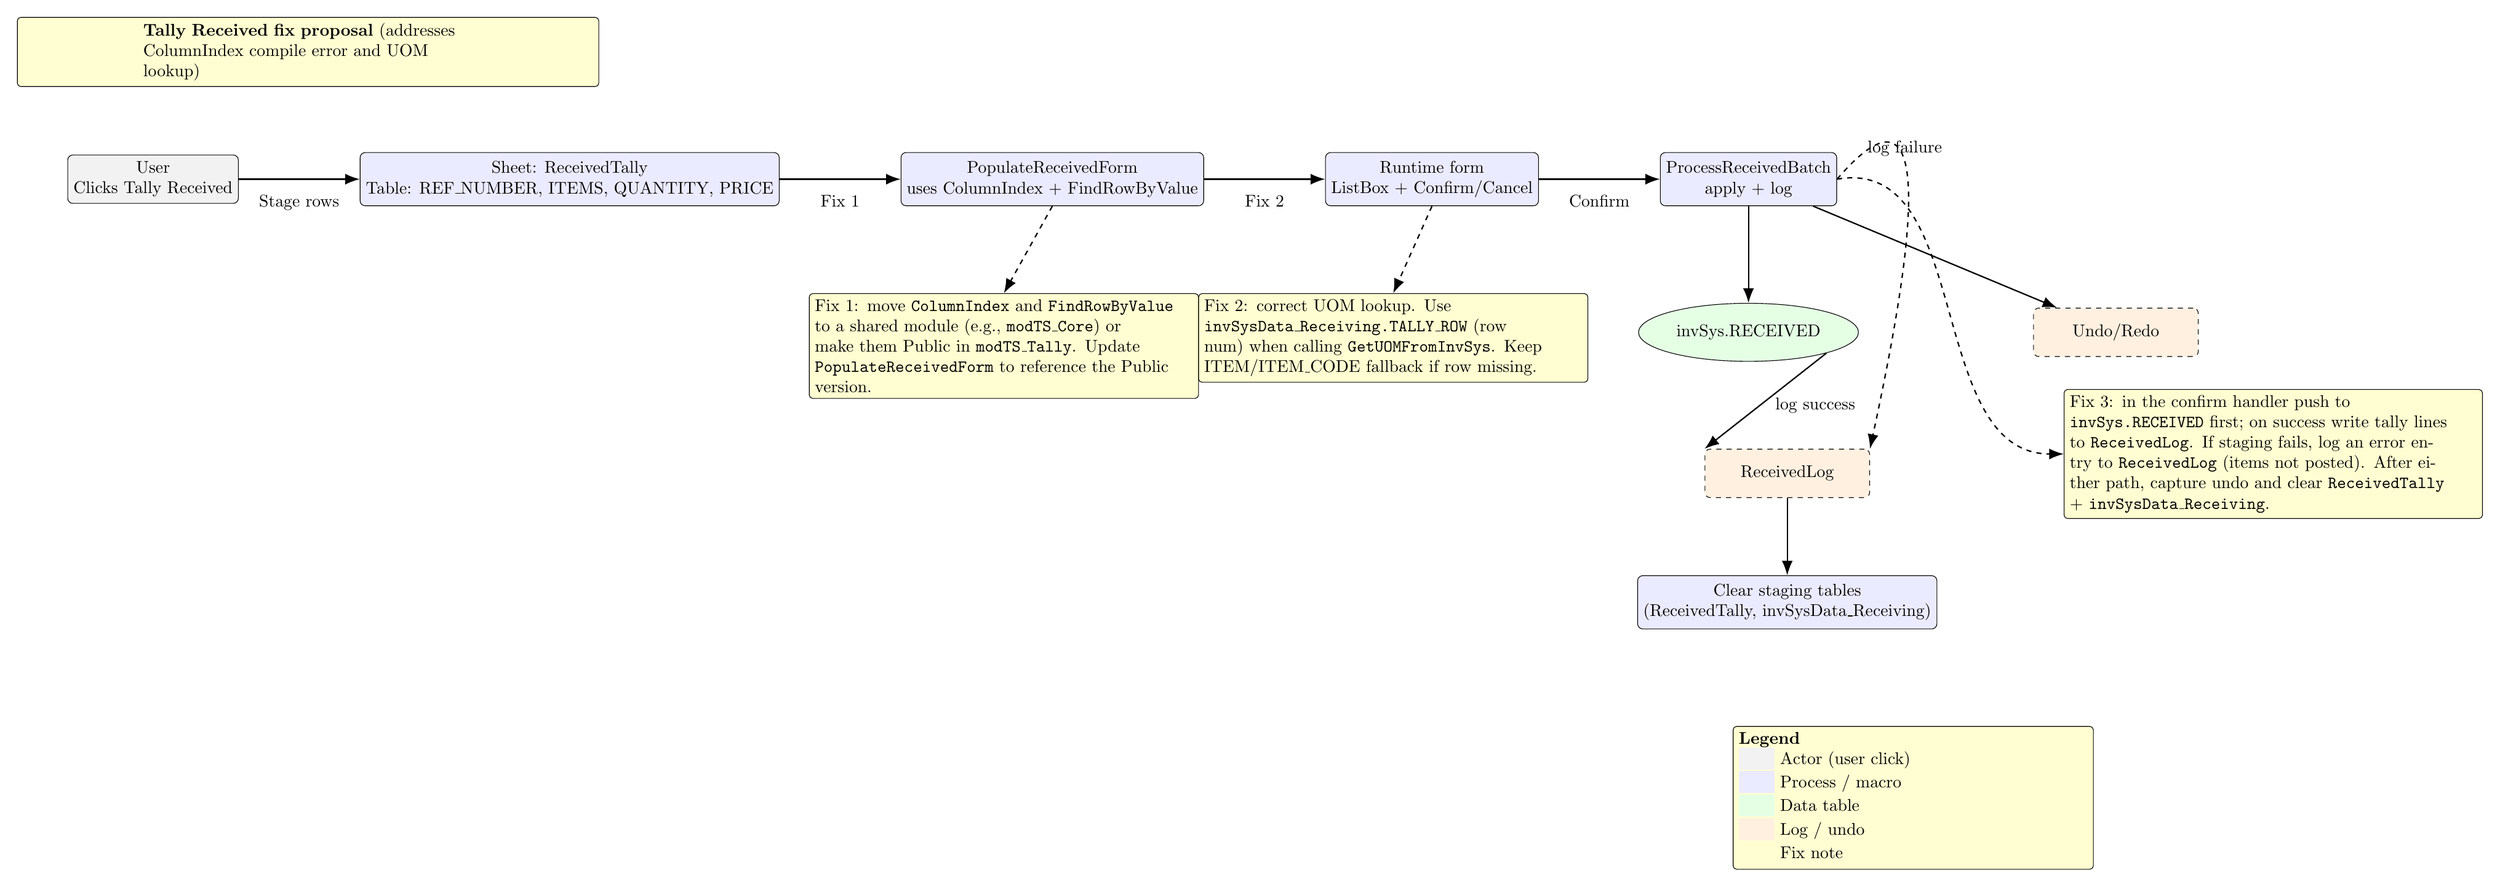
\begin{tikzpicture}[node distance=14mm]
  \node (title) [note,minimum width=120mm] {\textbf{Tally Received fix proposal} (addresses ColumnIndex compile error and UOM lookup)};

  \node (user) [actor,below=of title,xshift=-32mm] {User \\ Clicks Tally Received};
  \node (rt) [process,right=25mm of user] {Sheet: ReceivedTally \\ Table: REF\_NUMBER, ITEMS, QUANTITY, PRICE};
  \node (prep) [process,right=25mm of rt] {PopulateReceivedForm \\ uses ColumnIndex + FindRowByValue};
  \node (form) [process,right=25mm of prep] {Runtime form \\ ListBox + Confirm/Cancel};
  \node (batch) [process,right=25mm of form] {ProcessReceivedBatch \\ apply + log};
  \node (inv) [data,below=of batch,yshift=-6mm] {invSys.RECEIVED};
  \node (rlog) [log,below=18mm of inv,xshift=8mm] {ReceivedLog};
  \node (clear) [process,below=16mm of rlog] {Clear staging tables\\(ReceivedTally, invSysData\_Receiving)};
  \node (undo) [log,right=36mm of inv] {Undo/Redo};

  \draw[arrow] (user) -- (rt) node[midway,below,yshift=-2mm]{Stage rows};
  \draw[arrow] (rt) -- (prep) node[midway,below,yshift=-2mm]{Fix 1};
  \draw[arrow] (prep) -- (form) node[midway,below,yshift=-2mm]{Fix 2};
  \draw[arrow] (form) -- (batch) node[midway,below,yshift=-2mm]{Confirm};
  \draw[arrow] (batch) -- (inv);
  \draw[arrow] (inv.south east) -- node[pos=0.55,right,xshift=2mm]{log success} (rlog.north west);
  \draw[arrow,dashed] (batch.east) .. controls +(24mm,28mm) and +(6mm,28mm) .. node[pos=0.35,above]{log failure} (rlog.north east);
  \draw[arrow] (rlog) -- (clear);
  \draw[arrow] (batch) -- (undo);

  \node (fix1) [note,below=18mm of prep,xshift=-10mm,minimum width=78mm,text width=78mm] {Fix 1: move \texttt{ColumnIndex} and \texttt{FindRowByValue} to a shared module (e.g., \texttt{modTS\_Core}) or make them Public in \texttt{modTS\_Tally}. Update \texttt{PopulateReceivedForm} to reference the Public version.};
  \node (fix2) [note,below=18mm of form,xshift=-8mm,minimum width=78mm,text width=78mm] {Fix 2: correct UOM lookup. Use \texttt{invSysData\_Receiving.TALLY\_ROW} (row num) when calling \texttt{GetUOMFromInvSys}. Keep ITEM/ITEM\_CODE fallback if row missing.};
  \node (fix3) [note,right=40mm of rlog,yshift=4mm,minimum width=84mm,text width=84mm] {Fix 3: in the confirm handler push to \texttt{invSys.RECEIVED} first; on success write tally lines to \texttt{ReceivedLog}. If staging fails, log an error entry to \texttt{ReceivedLog} (items not posted). After either path, capture undo and clear \texttt{ReceivedTally} + \texttt{invSysData\_Receiving}.};

  \draw[arrow,dashed] (prep.south) -- (fix1.north);
  \draw[arrow,dashed] (form.south) -- (fix2.north);
  \draw[arrow,dashed] (batch.east) to[out=10,in=180] (fix3.west);

  \node (legend) [note,below=20mm of clear,xshift=26mm,minimum width=72mm,text width=72mm] {\textbf{Legend}\\
    \colorbox{gray!10}{\phantom{XX}} Actor (user click)\\
    \colorbox{blue!8}{\phantom{XX}} Process / macro\\
    \colorbox{green!10}{\phantom{XX}} Data table\\
    \colorbox{orange!12}{\phantom{XX}} Log / undo\\
    \colorbox{yellow!18}{\phantom{XX}} Fix note
  };
\end{tikzpicture}

\vspace{8mm}

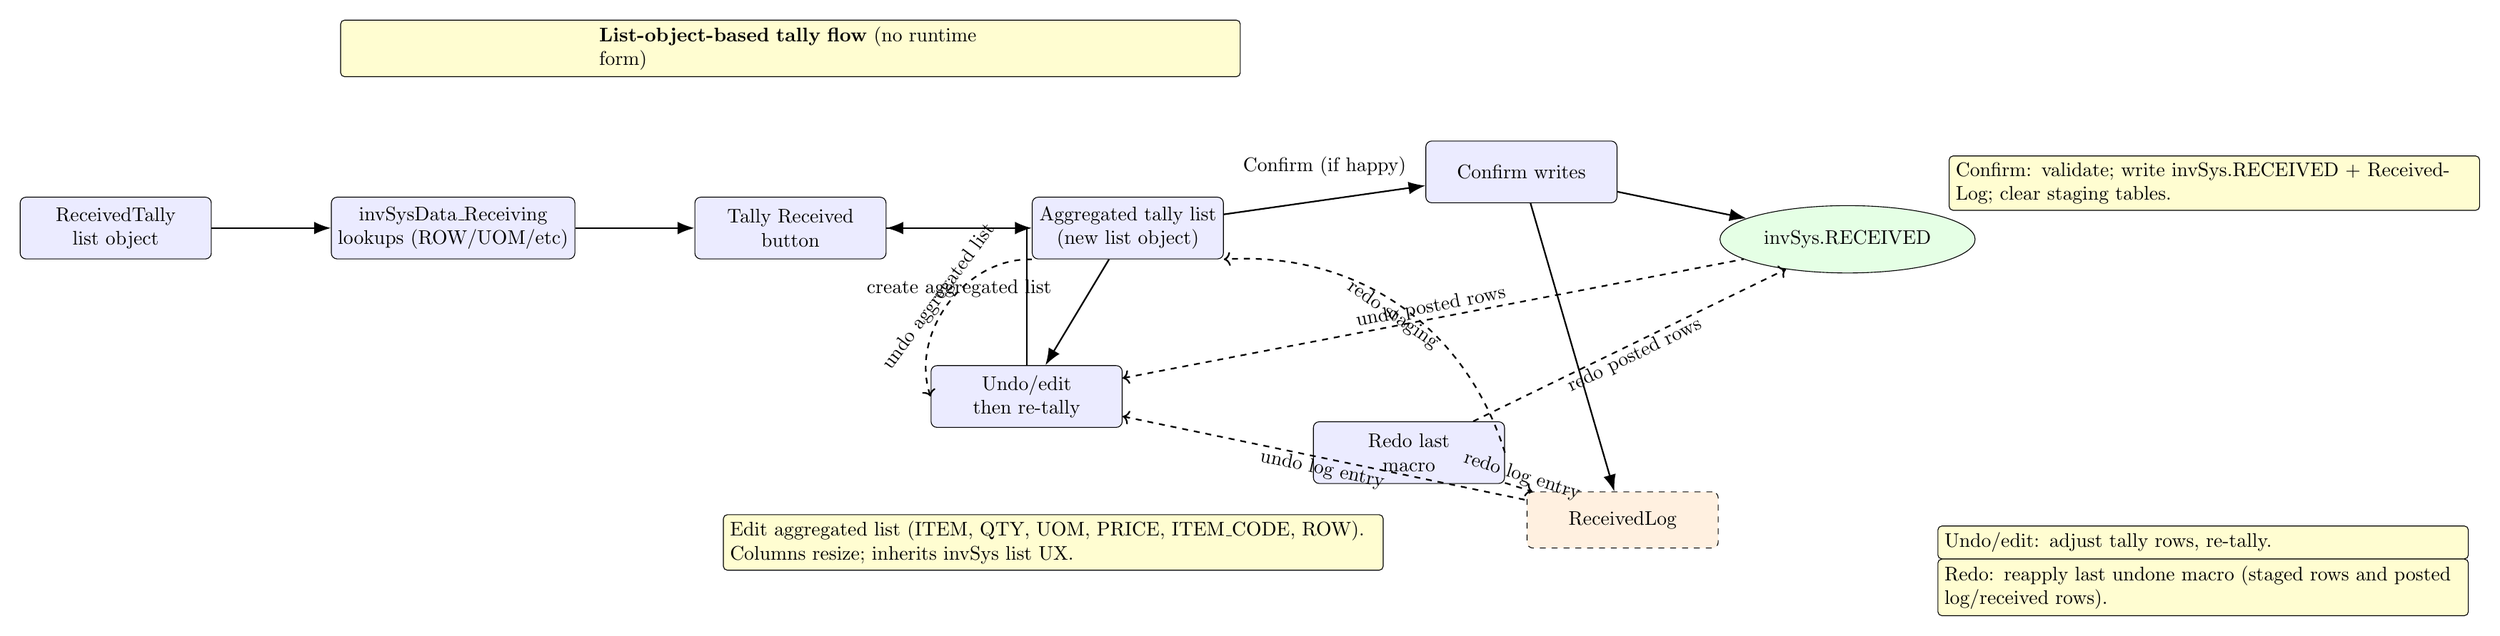
\begin{tikzpicture}[x=1mm,y=1mm]
  \node (title2) [note,minimum width=160mm] at (0,66) {\textbf{List-object-based tally flow} (no runtime form)};

  % main flow coordinates on a grid
  \node (rt2) [process] at (-120,34) {ReceivedTally \\ list object};
  \node (lookup) [process] at (-60,34) {invSysData\_Receiving \\ lookups (ROW/UOM/etc)};
  \node (tallybtn) [process] at (0,34) {Tally Received \\ button};
\node (agg) [process] at (60,34) {Aggregated tally list \\ (new list object)};
\node (confirm) [process] at (130,44) {Confirm writes};

\node (undo) [process] at (42,4) {Undo/edit \\ then re-tally};
\node (redo) [process] at (110,-6) {Redo last \\ macro};
\node (invwrite) [data] at (188,32) {invSys.RECEIVED};
\node (rlogwrite) [log] at (148,-18) {ReceivedLog};

\draw[arrow] (rt2) -- (lookup);
\draw[arrow] (lookup) -- (tallybtn);
\draw[arrow] (tallybtn) -- (agg);
\node[anchor=north] at (30,26) {create aggregated list};

\draw[arrow] (agg) -- (undo);
\draw[arrow] (agg) -- (confirm);
\node[anchor=south] at (95,42) {Confirm (if happy)};

\draw[arrow] (undo) |- (tallybtn);
\draw[arrow,bend left=15] (confirm) -- (invwrite);
\draw[arrow,bend right=30] (confirm) -- (rlogwrite);

% Macro-level undo paths (reverse arrows, dashed) to show we can roll back staging or posted writes
\draw[arrow,dashed,<- ,bend left=55] (undo.west) to node[above,sloped,inner sep=1pt]{undo aggregated list} (agg.south west);
\draw[arrow,dashed,<- ,bend right=30] (undo) -- node[above,sloped,inner sep=1pt]{undo posted rows} (invwrite);
\draw[arrow,dashed,<- ,bend right=12] (undo) -- node[below,sloped,inner sep=1pt]{undo log entry} (rlogwrite);
\draw[arrow,dashed,-> ,bend right=38] (redo.east) to node[below,sloped,inner sep=1pt]{redo staging} (agg.south east);
\draw[arrow,dashed,-> ,bend left=30] (redo) -- node[below,sloped,inner sep=1pt]{redo posted rows} (invwrite);
\draw[arrow,dashed,-> ,bend left=12] (redo) -- node[above,sloped,inner sep=1pt]{redo log entry} (rlogwrite);

\node[note,anchor=west,minimum width=115mm,text width=115mm] at (-12,-22) {Edit aggregated list (ITEM, QTY, UOM, PRICE, ITEM\_CODE, ROW). Columns resize; inherits invSys list UX.};
\node[note,anchor=west,minimum width=92mm,text width=92mm] at (206,42) {Confirm: validate; write invSys.RECEIVED + ReceivedLog; clear staging tables.};
\node[note,anchor=west,minimum width=92mm,text width=92mm] at (204,-22) {Undo/edit: adjust tally rows, re-tally.};
\node[note,anchor=west,minimum width=92mm,text width=92mm] at (204,-30) {Redo: reapply last undone macro (staged rows and posted log/received rows).};
\end{tikzpicture}

\vspace{8mm}

\end{document}
